\section{phase$\_$2}
	第二关的汇编代码如下:
	\begin{figure}[h]
		\centering
			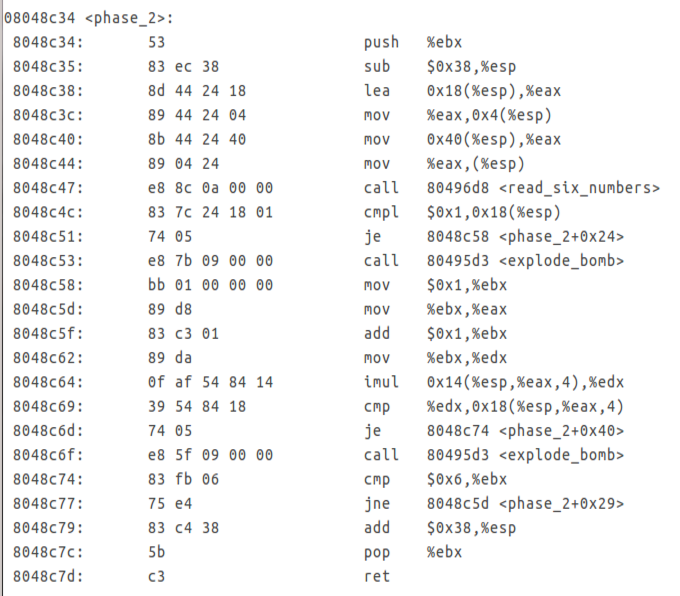
\includegraphics[scale=0.77]{images/phase_2.png}
	\end{figure}
	
	我们首先发现,它调用了一个\textbf{read$\_$six$\_$numbers}函数。经过分析,这个函数从输入中读入六个整数,并按地址从低到高存放在\textbf{0x18($\%$esp) - (0x30$\%$esp)}这24个字节中。也就是说,\textbf{a[0]}在\textbf{0x18($\%$esp)},\textbf{a[1]}在\textbf{0x1c($\%$esp)},以此类推。
	
	然后观察下面一段代码:
	
	\begin{figure}[h]
		\centering
			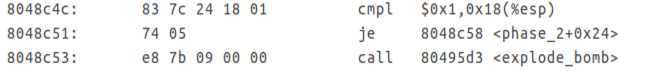
\includegraphics[scale=0.77]{images/phase_2_part_0.png}
	\end{figure}
	
	这段代码将\textbf{0x18($\%$esp)}即\textbf{a[0]}与$1$进行比较,如果不等则炸弹爆炸。这一段说明,我们输入的第一个数必须为1。
	
	接下来是一个循环:

	\begin{figure}[h]
		\centering
			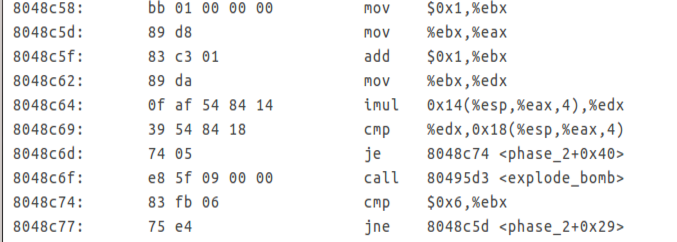
\includegraphics[scale=0.77]{images/phase_2_part_1.png}
	\end{figure}
		
	这个循环的循环变量是\textbf{$\%$ebx},从2循环到 5。同时, \textbf{$\%$eax}始终为
\textbf{$\%$ebx - 1}
	中间的判断语句,可以发现它是将\textbf{0x14($\%$esp, $\%$eax, 4) * $\%$edx}相乘,并与\textbf{0x18($\%$esp, $\%$eax, 4)}比较。由于a数组的起始位置为\textbf{0x18($\%$esp)}, 这两个地址就是\textbf{a[$\_$eax - 1]}和\textbf{a[$\_$eax]}。

	因此,其对应的c语言代码如下:

	\lstinputlisting{sources/phase_2.txt}
	
	这个函数表明,我们输入的数组a要满足以下条件:
	\begin{itemize}
		\item	数组长度为6
		\item	a[0] = 1
		\item	a[i] = a[i - 1] * (i + 1)
	\end{itemize}

	所以,第二关的答案就水落石出了: \textbf{1 2 6 24 120 720}
	
	考察知识点:数组的存储	